\chapter{Introduction}

The standard model (SM) gathers the entire understanding about fundamental particles and their interactions. Although the model has successfully explained various physical phenomena observed experimentally, there are still multiple unanswered questions concerning particle physics. For example, experiments \cite{Detectores} have shown that accelerator and reactor, solar, and atmospheric neutrinos have mass by proving the existence of neutrino oscillations. The fact that there are neutrino oscillations contradicts the SM, because this model precits that the neutrinos are massless. Some specific experiments for each neutrino category are: Super-Kamiokande \cite{Super-Kamiokande} for solar and atmospheric neutrino oscillations, KamLAND \cite{KamLAND} for reactor neutrinos, and K2K \cite{K2K} for accelerator neutrino oscillations \cite{Experimentos}. An additional open question about neutrinos is the fact that only neutrinos with left helicity have been observed. Helicity is defined as the projection of the particle's momentum vector over its spin direction. Only neutrinos with spin anti-parallel to its linear momentum have been observed.

In order to provide neutrinos with mass, several theories that extend the predictions of the SM have been proposed. One of the most known models is the "see-saw" or balance mechanism \cite{See-saw}. The see-saw mechanism includes three sub-models that provide mass to neutrinos. In this model, $\Phi = (\phi^{+}, \phi^{0})^{T}$ is the doublet associated with the SM Higgs Boson and $L_{l}$ the representation of a doublet field associated with the lepton number +1. In the type I see-saw mechanism the product between $L_{l}$ and $\Phi$ results in a fermionic singlet state. In the type II see-saw mechanism, the product between the two elements forms a scalar triplet. Finally, the product between $L_{l}$ and $\Phi$ in the type III sub-model results in a fermionic triplet state. Besides the see-saw mechanism, other models propose the existence of neutrinos with high mass and right helicity. If this kind of neutrinos are observed, the left and right symmetry in the SM would be restored and the mechanism by which the neutrinos acquire mass would be explained.

Heavy neutrinos searches have been conducted in experiments LEP \cite{LEP}, CMS and ATLAS \cite{CMS ATLAS}, but none of these collaborations has proved that heavy neutrinos exist. In order to understand heavy neutrino searches it is necessary to define the concept of jet. A jet at phenomenological level is defined as a quark or a gluon. In high energies experimental physics, a jet is defined as a collection of particles resulting from the fragmentation of quarks or gluons. Searches at CMS and ATLAS have focused in final states with associated leptons and jets. Figure \ref{fig: W} shows a Feynman diagram of the production of a heavy neutrino mediated by a W boson with left or right helicity. The final state for this process has two leptons ($\mu$ or $\tau$) and two jets.

\begin{figure}[H]
\centering
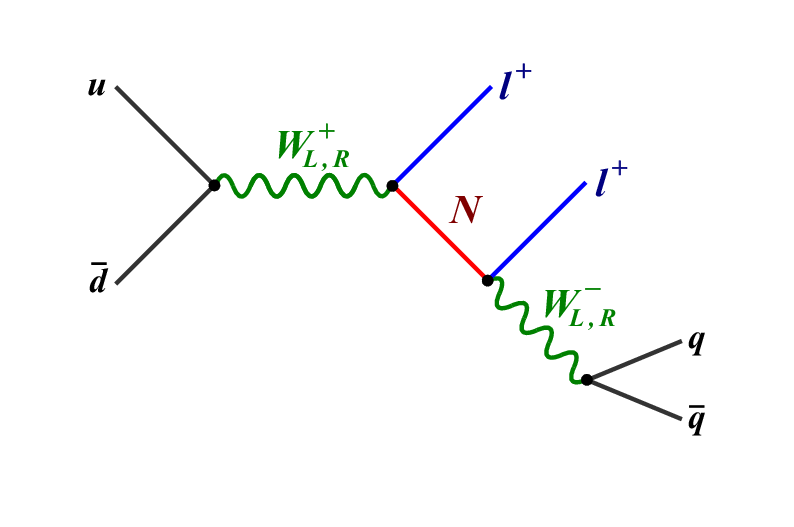
\includegraphics[width=\linewidth]{Figures/Feynman_W.png}
\caption{Feynman diagram of heavy neutrino production. (Taken from \cite{CMS ATLAS})}
\label{fig: W}
\end{figure}

The main objective of this monograph is to perform a phenomenological study about the feasibility of conducting an experimental analysis for the detection of heavy neutrinos in the Large Hadron Collider (LHC) using a technique known as vector boson fusion (VBF). This technique has been recently used in the LHC \cite{VBF Search} in searches for new physics. In high energy physics, the bosons $W^{\pm}$, $Z^{0}$ and $\gamma$ are known as vector bosons. The process of vector boson fusion occurs through an electroweak interaction of associated quarks with the LHC proton beams. In the analysis, the production of heavy neutrinos is considered through the decay of a high mass hypothetical resonance known as $Z^{'}$ (shown in the Feynman diagram of Figure \ref{fig: VBF}). This high mass resonance comes from the vector boson fusion process.

\begin{figure}[H]
\centering
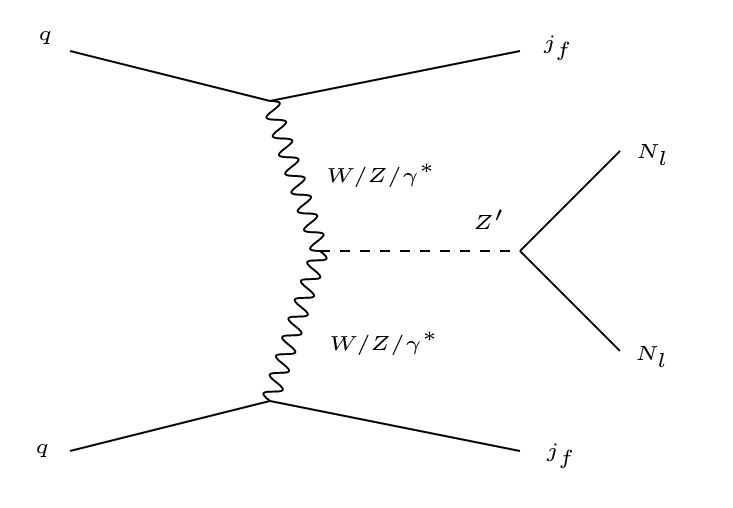
\includegraphics[scale = 0.65]{Figures/Feynman_VBF.JPG}
\caption{Feynman diagram of VBF process.}
\label{fig: VBF}
\end{figure}

The production of the heavy neutrino consists in the interaction of two quarks associated to the protons colliding in the beam. The protons emit vector bosons that produce a heavy resonance when they fuse. The heavy resonance decays afterwards producing the heavy neutrinos ($N_{l}$): $pp \rightarrow jj Z^{'} \rightarrow jj N_{l}N_{l}$.

The VBF topology consists in requiring two highly energetic jets in the longitundinal region of the detector and in opposite hemispheres thereof. It has been shown that by requiring this type of event, the noise level (background) is reduced considerably in regions of difficult study in searches of new physics.


In order to conduct the analysis, it is important to simulate signal and background processes and to perform a detailed physical study of the variables that allow to distinguish signal for experimental noise. It is necessary to use a cuantitative estimator commonly known as figure of merit to determine optimal cuts in the mentioned variables. The latter with the objective of reducing the amount of experimental noise by finding the optimal cuts in the relevant variables. For this particular analysis, the significance formula that will be used is the one shown in Equation 1, where $S$ is the significance, $N(s)$ is the number of signal events, and $N(B)$ is the number of background events.

\begin{equation}
    S = \frac{N(s)}{\sqrt{N(s) + N(B)}}
\end{equation}

Furthermore, it is important to establish the expected experimental sensitivity using maximum likelihood limits or the calculation of the final significance for different hypothetical signal points. The procedure described would allow to conclude whether a study for the detection of heavy neutrinos at the LHC is feasible or not.
